\section{Problem 1}
\textit{Using the overhearing cross topology for NC, consider that transmission of a packet has a cost of $E_t$ and reception of a packet a cost of $E_r$. Assume initially no losses in the links.}\\


\textbf{Note that the \textcolor{gray}{gray} colored parts in the following is a part of problem 2.}

\begin{figure}[h!]
  \centering
  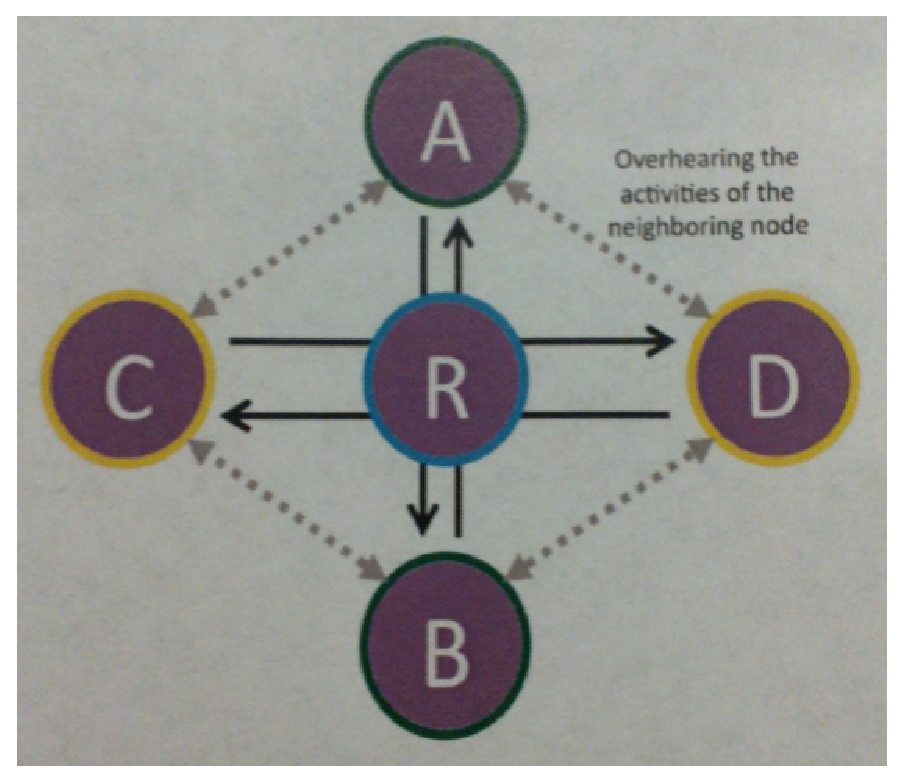
\includegraphics[width=8cm]{MM10_thecross.eps}
  \caption{The butterfly cross}
  \label{fig:MM12_thecross}
\end{figure}
\FloatBarrier

\subsection{a)} 
\textit{Calculate the total energy used to deliver one packet from each source (A,B,C,D) to its intended receiver (B, A, D, C, respectively) at each of the network's nodes when using network coding versus no coding (forwarding). Leave this cost in terms of $E_t$ and $E_r$}

\begin{table}[h!]
  \centering
  \begin{tabular}{|r|c|c|c|c|}
    \hline
          & \multicolumn{2}{c|}{No Coding:} & \multicolumn{2}{c|}{Network Coding} \\
          & R:    & Nodes: & R:    & Nodes: \\ \hline
    Trans. & 4     & 1     & 1     & 1 \\
    Recep. & 4     & 1     & 4     & 3 \\    \hline
          & 4$E_t$+4$E_r$ & $E_t$+$E_r$ & $E_t$+4$E_r$ & $E_t$+3$E_r$ \\
          &			& \textcolor{gray}{+6$E_{idel}$}& \textcolor{gray}{+$E_{XOR}$} & \textcolor{gray}{+$E_{idel}$+$E_{XOR}$} \\	
    \hline
  \end{tabular}%
  \caption{Energy needed for reception ($E_r$) and transmission ($E_t$)} \label{tab:addlabel}%
\end{table}%

\FloatBarrier
\subsection{b)} 
\textit{Using the results from a), calculate the overall energy (OE) of the system for both network cording and forwarding.}\\
 
$OE = E_{Relay}+4E_{node}$
\subsubsection{With No Coding:}
$OE_{NC} = 4E_t+4E_r+4E_t+4E_r\textcolor{gray}{+24E_{idel}}$
$OE_{NC} = 8\left(E_t+E_r\textcolor{gray}{+3E_{idel}}\right)$
\subsubsection{With Network Coding:}
$OE_{WC} = E_t+4E_r+4\left(E_t+3E_r\right)\textcolor{gray}{+4E_{idel}+5E_{XOR}}$
$OE_{WC} = 5E_t+16E_r\textcolor{gray}{+4E_{idel}+5E_{XOR}}$

\FloatBarrier
\subsection{c)} 
\textit{Calculate the energy per transmitted packet in the system for both communication schemes.}

\subsubsection{With No Coding:}
$\frac{Energy}{Packet}=\frac{OE_{NC}}{4}$
$\frac{Energy}{Packet}=2\left(E_t+E_r\textcolor{gray}{+3E_{idel}}\right)$
\subsubsection{With Network Coding:}
$\frac{Energy}{Packet}=\frac{OE_{WC}}{4}$
$\frac{Energy}{Packet}=\frac{5}{4}E_t+4E_r\textcolor{gray}{+E_{idel}+\frac{5}{4}E_{XOR}}$

\FloatBarrier
\subsection{d)} 
\textit{Calculate the packet delivery energy per throughput rate for both communication schemes.}\\

Throughput Rate (TP) $TR=\frac{Packet transmitted}{\# time slots}$
\subsubsection{With No Coding:}
$TR=\frac{4}{8}=\frac{1}{2}$
$\frac{Energy per Trace}{TR}=4\left(E_t+E_r\textcolor{gray}{+3E_{idel}}\right)$
\subsubsection{With Network Coding:}
$TR=\frac{4}{5}$
$\frac{Energy per Trace}{TR}=E_t+5E_r\textcolor{gray}{+\frac{5}{4}E_{idel}+E_{XOR}}$

\FloatBarrier
\subsection{e)} 
\textit{Given the previous results, in there a set of $E_t$ and $E_r$ pairs where network coding performs worse in terms of the different metrics presented in b) - d) ? By creating a plot with $E_t$ in the x-axis and $E_r$ in the y-axis for each of the three metrics, show the regions of operation where each scheme is useful.}

\begin{figure}[h!]
  \centering
  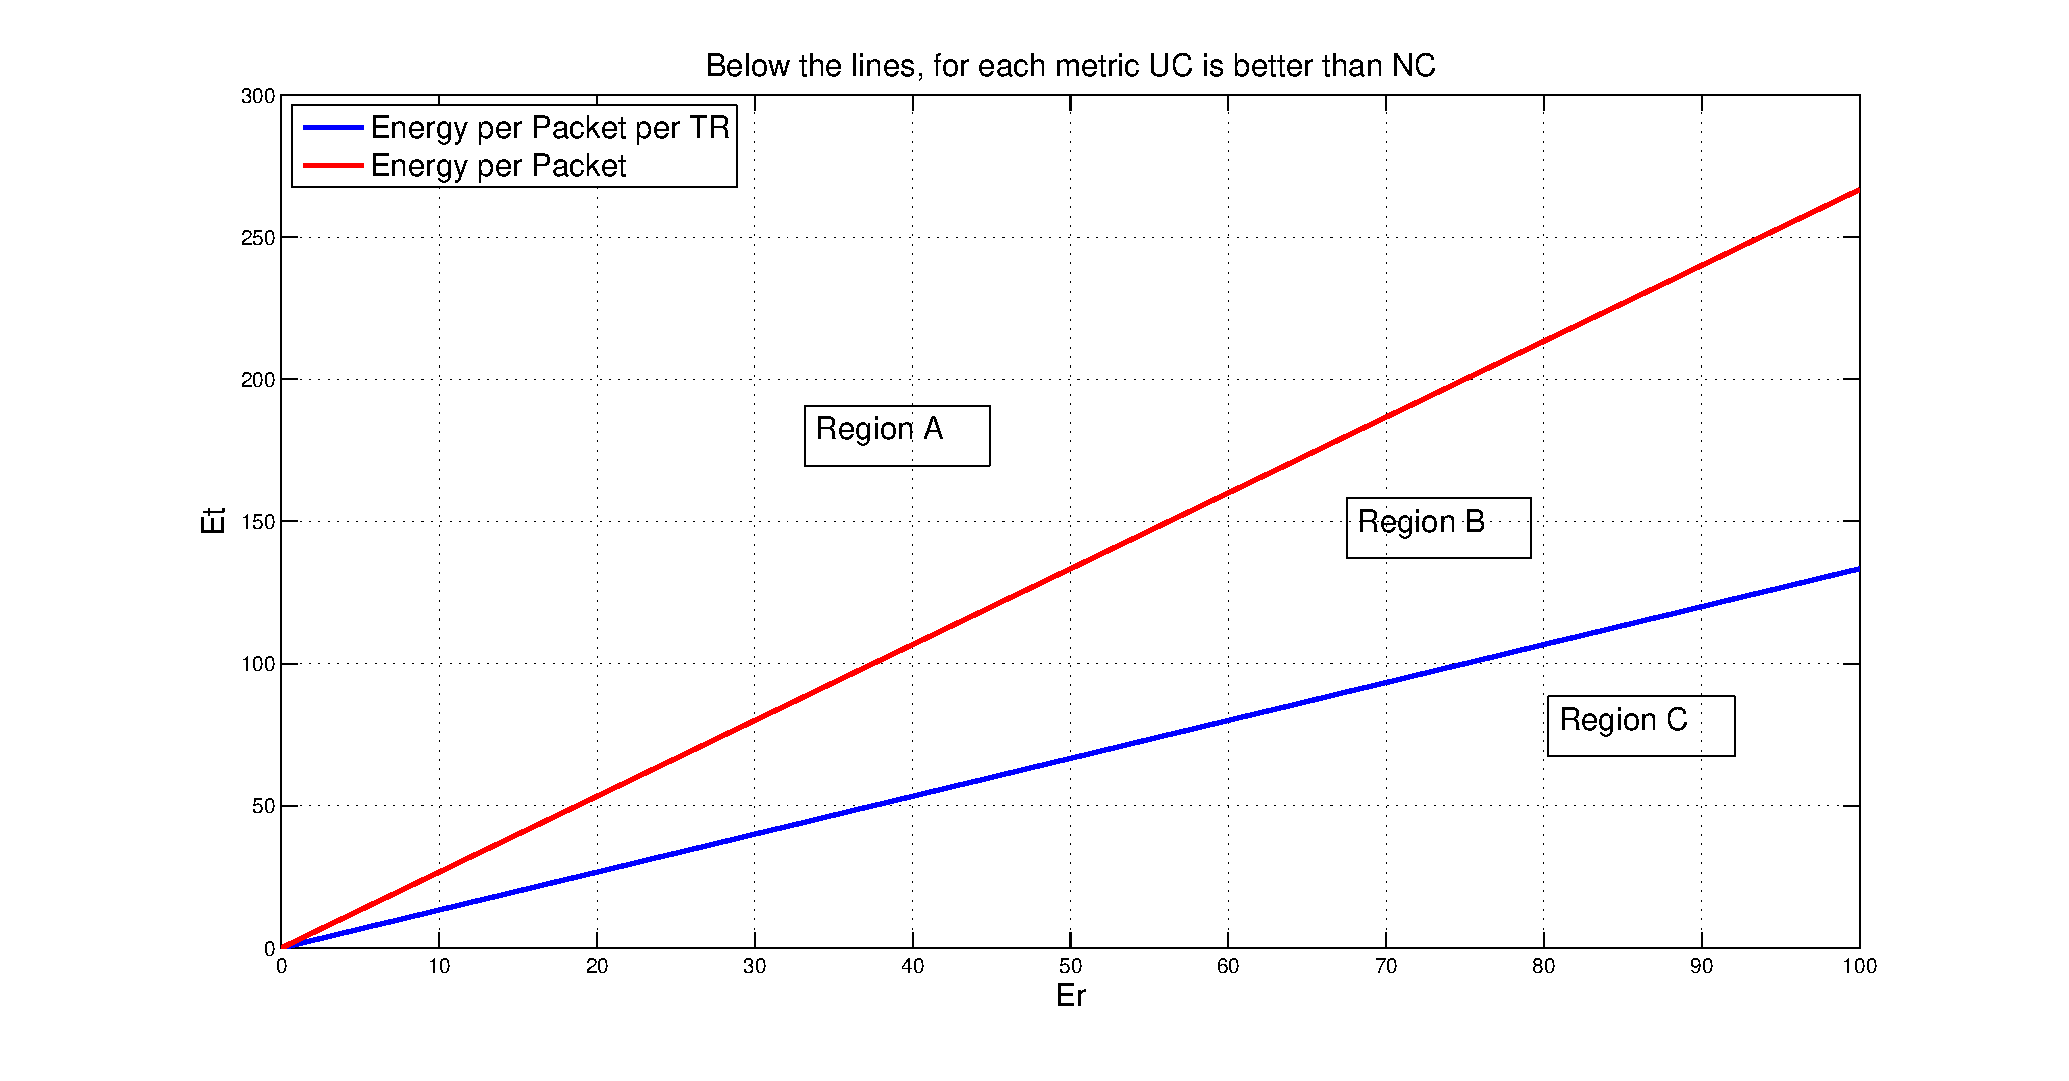
\includegraphics[width=18cm]{mm11_exc_1_d_plot_1.eps}
  \caption{Plot 1}
  \label{fig:mm11_exc_1_d_plot_1}
\end{figure}

\begin{figure}[h!]
  \centering
  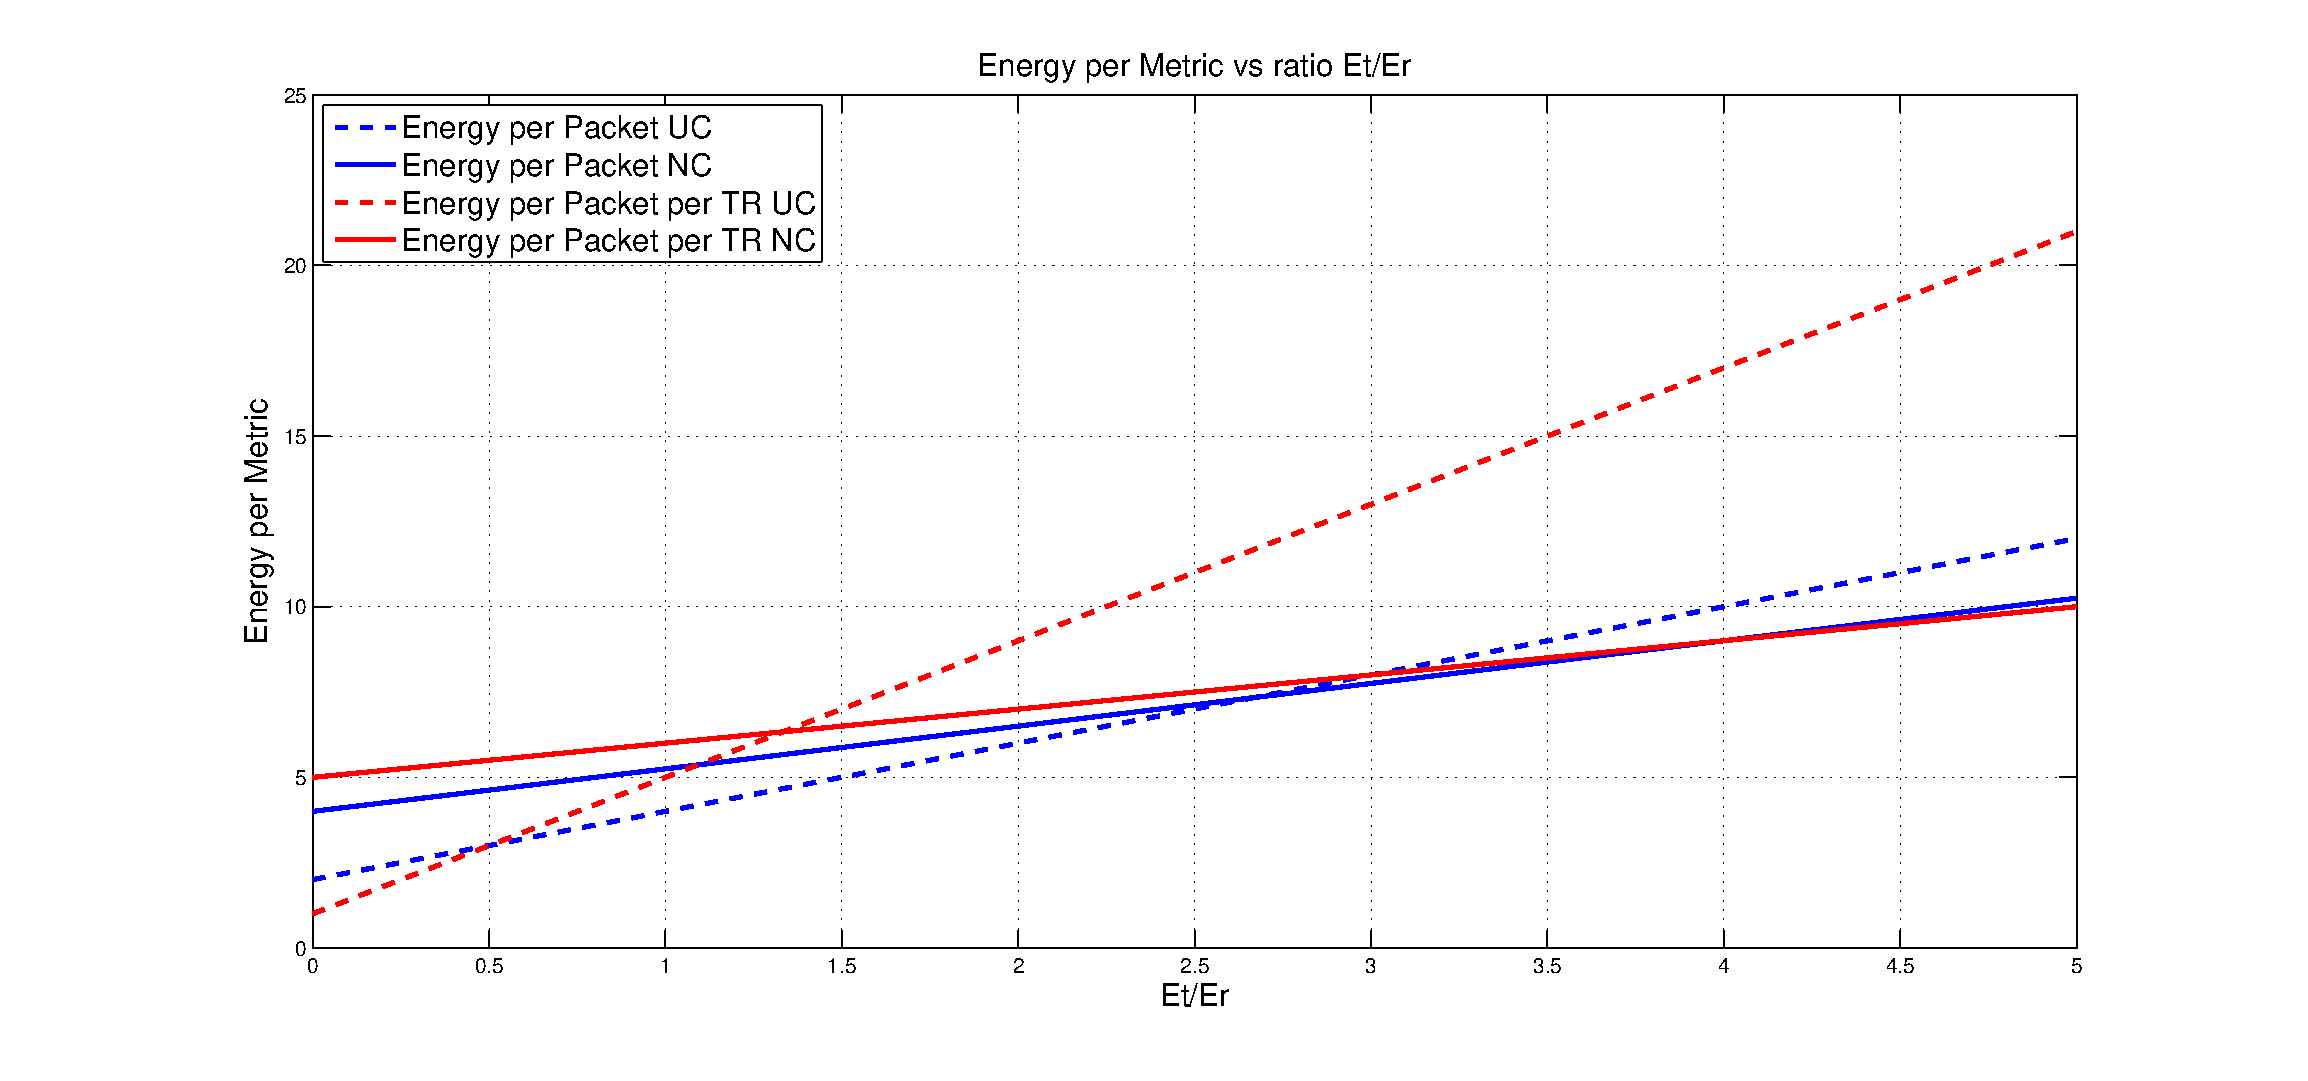
\includegraphics[width=18cm]{mm11_exc_1_d_plot_2.eps}
  \caption{Plot 2}
  \label{fig:mm11_exc_1_d_plot_2}
\end{figure}

\FloatBarrier
Metric will be the following:
\begin{pitemize}
	\item Uncoded is better when: $E_t\leq\frac{8}{3}E_r$
	\item Coded is better when: $E_t\leq\frac{4}{3}E_r$
\end{pitemize}


